% !TEX root = ../ac_paper.tex

\section{Introduction\label{sec:intro}}

We live in an extraordinary era where artificial intelligence (AI) is transforming numerous sectors and professions. Recent advancements in Large Language Models (LLMs) have empowered AI to read, write, and converse with a proficiency comparable to that of human experts. In the realm of board games, AI has outperformed even the most skilled human players, and it has tackled complex scientific challenges like protein folding, where steady progress was suddenly overtaken by a near-complete solution. As AI continues to evolve, one critical question remains: How wide is the range of domains in which AI systems can reason as effectively as humans?

Mathematics appears to be a natural progression on the path toward Artificial General Intelligence (AGI) due to its universal syntactic and logical structure, similar to that of natural language. Additionally, mathematics provides a framework for the quantitative evaluation of logical and analytical reasoning, making it an ideal domain for self-improving AI systems on the path to AGI. In a moment, we will explain another reason why mathematics could play a crucial role in AGI development, but first, we need to introduce one more key element: reinforcement learning (RL).

Machine learning, a subfield of AI, involves developing algorithms and statistical models that enable computers to learn from data and make predictions. Among the three primary areas of machine learning---supervised learning, unsupervised learning, and reinforcement learning---RL emphasizes learning through interaction with an environment and receiving feedback in the form of rewards or penalties. This aspect of machine learning, often characterized by its focus on AI models `playing games,’ will be central to our discussion.

A typical chess game lasts about 30 to 40 moves, with the longest recorded professional game reaching 269 moves, ending in a draw between Ivan Nikolic and Goran Arsovic in 1989. Notably, the number of moves in a typical chess game is relatively consistent, with the longest professional game having only about an order of magnitude more moves than the average. Similarly, a typical game of Go involves a few hundred moves, with the longest recorded professional game, played by Go Seigen and Kitani Minoru in 1933, lasting 411 moves.

At first glance, proving or disproving mathematical conjectures can be formulated as games. For example, proving a theorem involves finding a path from the hypothesis to the conclusion, consisting of basic logical steps, such as Lean steps. From the RL perspective, this type of game can be quite complex due to its large action space. Conversely, finding examples or counterexamples to settle important conjectures may require only a few basic moves (actions); the case study in this paper serves as a good illustration of such a problem. In all cases, the problem is fundamentally a search process, with complexity largely determined by the size of the action space and the search space.

In addition, with hard research-level mathematics problems, one faces yet another challenge: the sought-after instance can be so rare and difficult to find that the problem effectively becomes a search for a needle in a haystack, i.e., a problem with ultra-sparse rewards. For example, in the context of theorem proving, one might consider an extremely hard theorem\footnote{A proxy for such a problem could be the Riemann Hypothesis or any other unsolved Millennium Prize Problem.} that may require a very large number of steps. If there aren't many alternative proofs, finding even a small number of very long ones then becomes akin to searching for a needle in a haystack or, depending on one's preference, a search for a unicorn.\footnote{Similar challenges, though not as critical, also arise in non-research-level math problems; see, e.g., \cite{peano,dabelow2024symbolicequationsolvingreinforcement,trinh2024solving} for recent discussion. Meanwhile, in a parallel line of development, new benchmarks have been proposed in the past couple of years \cite{procgen,NeedleInAHaystack}, which can be useful in such contexts.}

Fortunately, mathematics offers a robust framework for developing and testing new algorithms with adaptive capabilities that dynamically `learn how to learn.' Testing these algorithms on mathematical problems, rather than directly on societal issues like market crash predictions or extreme weather events, provides a risk-free and cost-effective approach. Additionally, this method offers the dual benefit of potentially solving hard mathematical problems and resolving long-standing conjectures in the process.

Our approach to problems of this type involves equipping the RL model with the ability to assess the hardness of problems during the training process. First and foremost, this requires a practically useful notion of hardness, a concept we thoroughly explore. By learning the distribution of problems based on their difficulty, one can enhance existing off-the-shelf algorithms with new self-improvement strategies, identifying key features that facilitate solving the most challenging problems.

In this paper, we begin a systematic implementation of this approach by carefully analyzing the distribution of hardness in potential counterexamples to a long-standing conjecture, the Andrews--Curtis conjecture. As with many other challenging problems, a natural measure of hardness is the number of steps an RL agent needs to take. What makes the Andrews--Curtis conjecture particularly suitable for our study is that it includes numerous examples requiring a hyper-exponential number of steps, providing an effective testbed for exploring the aforementioned questions through the lens of RL, search algorithms, and topological data analysis.

We should emphasize that this entire project was carried out using relatively modest computational resources that a small academic research group can easily afford. Consequently, we placed greater emphasis on theoretical tools and techniques that, when combined with scaled-up computational resources, can lead to further advancements.

While our primary focus is on exploring the distribution of hardness with an eye toward algorithm development, we also resolve a number of particularly interesting open cases that has eluded direct mathematical approaches for decades. Below we provide a few explicit examples.

\begin{theorem}\label{thm:MS}
The following potential counterexamples introduced by Miller and Schupp \cite{Miller--Schupp} are AC-trivial:
\begin{equation}
\angles{x, y \mid x^{-1} y^3 x y^{-4} , \ x^{-1} y^{-1} x^{-1} y^{-1} x y^{-3} }
\end{equation}
\begin{equation}
\angles{x, y \mid x^{-1} y^4 x y^{-5} , \ x^{-1} y x y^{-1} x^{-1} y^{-3} }
\end{equation}
\end{theorem}

\medskip\noindent
In addition, motivated by the work \cite{MMS}, where it was argued that the following length 25 presentation
\begin{equation}\label{eq:MMS3}
\angles{ x, y \mid
	x^{-1}y^{-1}xy^{-1}x^{-1}yxy^{-2}xyx^{-1}y, \
	y^{-1}x^{-1}y^2x^{-1}y^{-1}xyxy^{-2}x }
\end{equation}
is part of a family of stably AC-trivial presentations, we established its equivalence to another prominent presentation introduced by Akbulut and Kirby \cite{Akbulut--Kirby}.

\begin{theorem}\label{thm:stableAK3}
	The following potential counterexample introduced by Akbulut and Kirby \cite{Akbulut--Kirby} is AC-equivalent to :
	\[
	\AK(3) = \angles{x, y \mid x^3 = y^{4}, xyx = yxy}.
	\]
\end{theorem}

\medskip\noindent
The initial preprint of this paper stimulated significant developments. In particular, a subtle misprint that escaped the notice of referees was found in \cite{MMS} more than 20 years since its publication, making \eqref{eq:MMS3} {\it not} stably AC-trivial. The original result, establishing equivalence to $AK(3)$ in theorem \ref{thm:stableAK3} is still correct. And we hope that the status of $AK(3)$ will be resolved in the near future with the help of the methods introduced in this paper.
%
The proofs of theorems \ref{thm:MS} and \ref{thm:stableAK3} are presented in \autoref{sec:RLsolutions}.

The rest of the paper is organized as follows. In \autoref{sec:AC}, we provide an overview of the Andrews--Curtis conjecture, describing the specific version studied in this work. We then apply classical search algorithms to examples in the Miller--Schupp series in \autoref{sec:search}, where we devise a greedy search algorithm that significantly outperforms the widely used breadth-first search algorithm. In \autoref{sec:rl}, we employ reinforcement learning, specifically implementing the Proximal Policy Optimization (PPO) algorithm \cite{schulman2017proximal}, and find that while it performs better than breadth-first search, it does not surpass the greedy search algorithm (see \autoref{fig:performance}). Building on these insights, \autoref{sec:algo} presents several ideas for algorithm development, proposing strategies to mitigate the overwhelming complexity faced by an RL agent in challenging problems. In \autoref{sec:isolated}, we employ topological methods to assess the complexity of presentations. Specifically, we utilize persistent homology to define the \textit{isolation value} of a presentation. This value is infinite for counterexamples to the AC conjecture and serves as a measure of a presentation's resistance to being trivialized. Finally, in \autoref{sec:lm}, we examine the linguistic structure of balanced presentations using a decoder-only Transformer model, observing distinct clusters within the embedding space corresponding to presentations solved and unsolved by the greedy search algorithm.

\medskip\noindent
We encourage the reader to explore the accompanying GitHub repository:
\begin{center}
	\href{https://github.com/shehper/AC-Solver}{https://github.com/shehper/AC-Solver}\todo{Add URL to the comments section of the arXiv's metadata.}
\end{center}

\begin{figure}
	\centering
	\begin{subfigure}[b]{0.5\textwidth}
		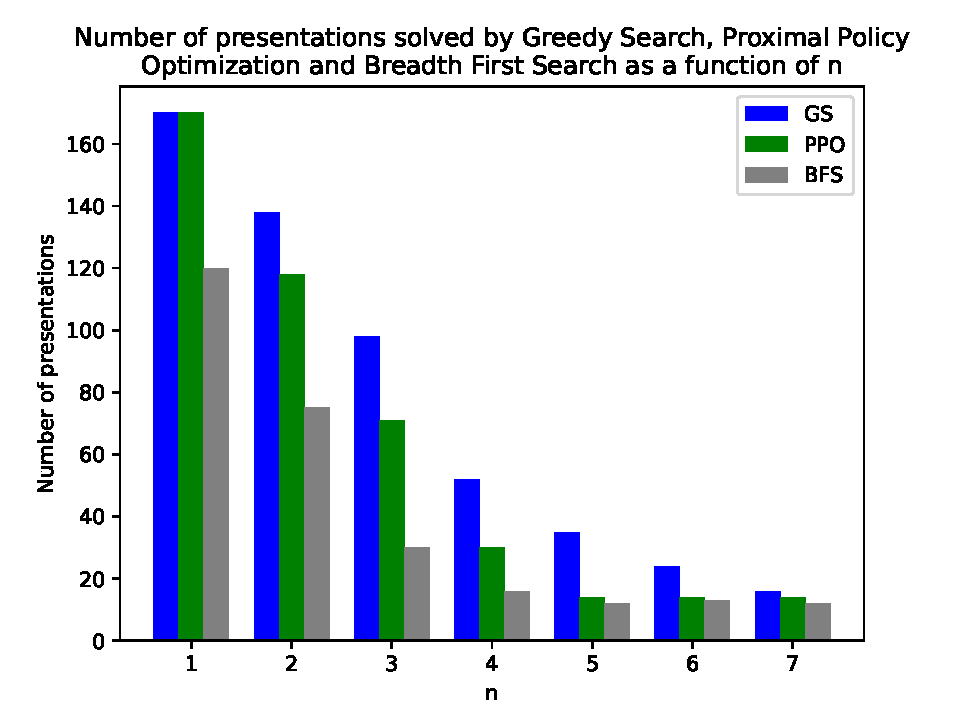
\includegraphics[width=1.1\textwidth]{fig/performance_vs_n.pdf}
		\caption{Distribution versus $n$}
		\label{fig:performance_vs_n}
	\end{subfigure}
	\begin{subfigure}[b]{0.5\textwidth}
		\centering
		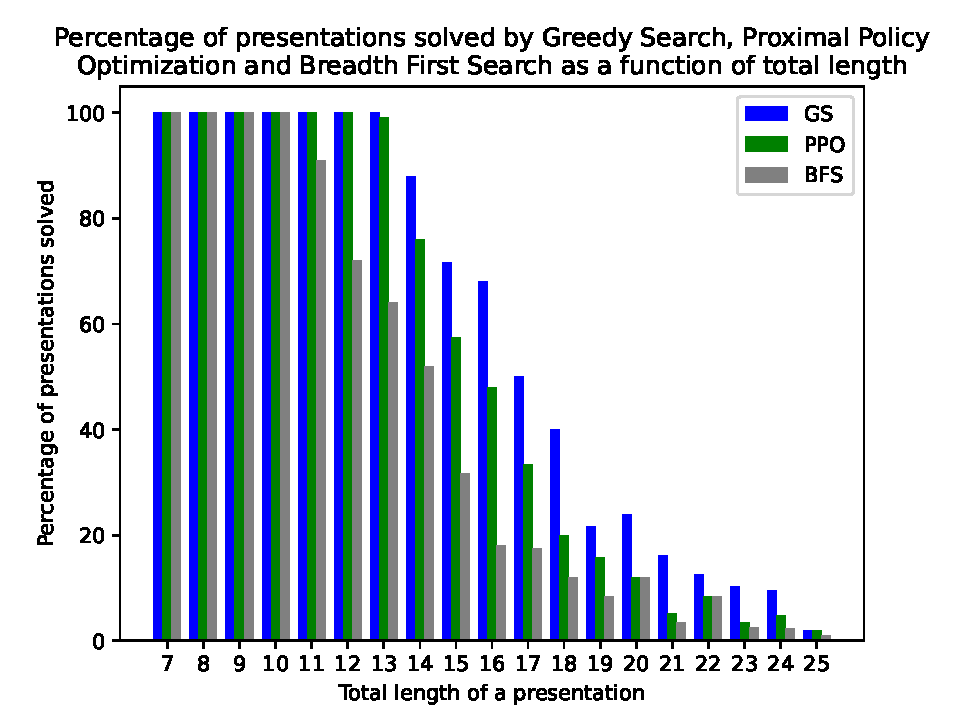
\includegraphics[width=1.1\textwidth]{fig/performance_vs_length.pdf}
		\caption{Distribution versus length}
		\label{fig:performance_vs_length}
	\end{subfigure}
	\caption{A comparison of three algorithms ---breadth-first search, greedy search, and Proximal Policy Optimization (PPO)--- that we used to search through the space of balanced presentations. The number of presentations of the Miller--Schupp series, $\MS(n, w)$, solved by an algorithm is given on the vertical axis. We compare the performance as a function of $n$ (above) and the length of the presentation (below). Greedy Search consistently outperforms Breadth-First Search and Proximal Policy Optimization.}
	\label{fig:performance}
\end{figure}